\section*{Теория}
Голография -- способ записи изображения, который позволяет по картине интенсивности восстановить полную информацию о волновом поле. Техника записи голограмм отображена на рис. 1. Важным свойством голограммы является возможность восстановить по её малому участку информацию обо всём объекте. 

\begin{figure}[tbp]	
	\centering
	\begin{minipage}{0.49\linewidth}
		\centering
		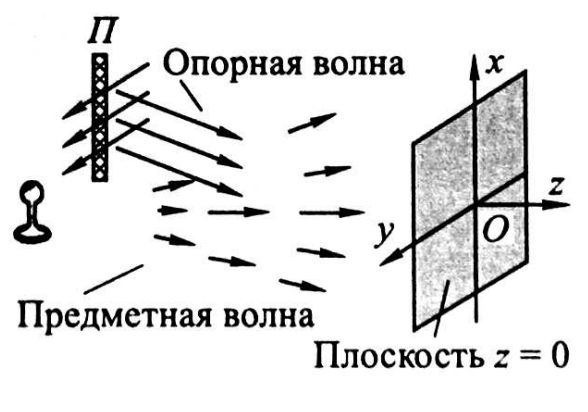
\includegraphics[width=0.8\linewidth]{../Изображения/Формирование.png}
		\caption{Запись голограммы}
	\end{minipage}
	\begin{minipage}{0.49\linewidth}
		\centering
		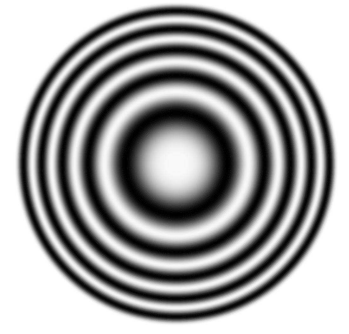
\includegraphics[width=0.8\linewidth]{../Изображения/Габор.png}
		\caption{Зонная решётка Габора}
	\end{minipage}
\end{figure}

Назовём волну, падающую на предмет, предметной; а волну, падающую сразу на плёнку -- опорной. Эти волны должны быть когерентны. Тогда:
\begin{equation*}\label{key}
	t \propto a^2+a_о^2+2 a a_o \cos (\varphi - \varphi_о),
\end{equation*}
то есть сохраняется информация о фазе волны.

В частности, для точечного источника, считая, что $ f_п = a e^{i k z}  $ и $ f_о \approx a e^{i k r} $, получаем голограмму  с функцией пропускания
\begin{equation*}\label{key}
	t(x, y) \propto \left| a+ a e^{i k r}\right|^2.
\end{equation*}

Для обратного процесса -- восстановления -- применяют плоскую нормально падающую волну. Считая $ f_- (x, y) \equiv 1, $ на выходе голограммы точечного источника получим:
\begin{equation*}\label{key}
	f_+ (x, y) = \left| a+ a e^{i k r}\right|^2 = 2 a^2 (1+\cos (k r)) = 2 a^2 + a^2 e^{i k r} +a^2 e^{- i k r}.
\end{equation*}
Отсюда видна структура полученной волны: суперпозиция плоской и двух сферических волн (соответствующих действительному и мнимому источникам).

Голограмма точечного источника имеет вид колец (рис. \ref{fig:screenshot1}) с радиусами
\begin{equation*}\label{key}
	\rho_m = \sqrt{m \lambda z_0},
\end{equation*}
где нечётному $ m $ соответствуют тёмные кольца.

Одним из свойств голограммы является её разрешающая способность, определяемая выражением:
\begin{equation*}\label{key}
	\Delta x \sim \frac{\lambda}{D} z_0,
\end{equation*}
где $ z_0 $ -- расстояние от источника до его голограммы, а $ D $ -- размер голограммы.


